\documentclass[12pt,a4paper]{article}

% --- Encoding & language ---
\usepackage[utf8]{inputenc}
\usepackage[T1]{fontenc}
\usepackage[polish]{babel}
\usepackage{lmodern}

% --- Math & symbols ---
\usepackage{amsmath,amssymb,amsthm}
\usepackage{mathtools}
\usepackage{bm}

% --- Layout ---
\usepackage[margin=2.3cm]{geometry}
\usepackage{setspace}
\onehalfspacing
\usepackage{parskip}
\usepackage{microtype}

% --- Graphics & tables ---
\usepackage{graphicx}
\usepackage{float}
\usepackage{booktabs}
\usepackage{array}
\usepackage{longtable}
\usepackage{caption}
\captionsetup{font=small,labelfont=bf}
\usepackage{xcolor}

% --- Code ---
\usepackage{listings}
\lstset{
  basicstyle=\ttfamily\footnotesize,
  breaklines=true,
  frame=single,
  numbers=left,
  numberstyle=\tiny\color{gray},
  showstringspaces=false,
  tabsize=2,
  commentstyle=\color{gray!70!black},
  keywordstyle=\color{blue!60!black}\bfseries,
  stringstyle=\color{green!50!black},
  language=Python
}

% --- Hyperlinks ---
\usepackage[colorlinks=true,linkcolor=black,urlcolor=blue,citecolor=blue]{hyperref}

% --- Header / footer ---
\usepackage{fancyhdr}
\pagestyle{fancy}
\fancyhf{}
\fancyhead[L]{\small \textit{Praca z danymi medycznymi: import, przetwarzanie i analiza}}
\fancyfoot[C]{\thepage}
\renewcommand{\headrulewidth}{0.4pt}

% --- Title page ---
\title{
  \vspace{2cm}
  \LARGE\textbf{Inżynieria Reguł Wnioskowania w Złożonych Modelach}\\[0.6cm]
  \Large Laboratorium 1\\[0.4cm]
  \large \textit{Praca z danymi medycznymi: import, przetwarzanie i analiza}\\[0.3cm]
  \normalsize Wariant: \textbf{1 (fallback z 8) — dataset 8: Prostate cancer (synth)}
}
\author{Jakub Jurzak 59099}
\date{07.05.2026}

\begin{document}
\maketitle
\thispagestyle{empty}
\newpage

\tableofcontents
\newpage

\section{Cel zadania}
Zapoznanie z procesem pracy z danymi medycznymi: importem, czyszczeniem, uzupełnianiem braków, standaryzacją, analizą statystyczną oraz wizualizacją danych pacjentów. W wariancie wykorzystano kohortę pacjentów onkologicznych (prostate cancer, syntetyczna).

\section{Opis problemu}
Dane medyczne są wrażliwe, niejednorodne i często niekompletne. Zadaniem jest ich przygotowanie do analizy oraz dalszego modelowania, w tym diagnoza braków, konwersja typów, standaryzacja zmiennych ilościowych oraz weryfikacja zależności między cechami a stanem klinicznym pacjenta.

\section{Opis danych}
Zbiór syntetyczny imitujący kohortę prostate-cancer-survival (N=600). Zmienne: \texttt{age}, \texttt{psa}, \texttt{gleason\_score}, \texttt{tumor\_stage}, \texttt{treatment}, \texttt{comorbidities}, \texttt{survival\_months}, \texttt{survived}. Braki danych wprowadzono losowo w kolumnie \texttt{psa} (5\%).

\section{Opis metod}
Zastosowano: (a) uzupełnianie braków medianą dla \texttt{psa}; (b) standaryzację Z-score zmiennych ilościowych; (c) statystyki opisowe (średnia, mediana, odch.\ std., min, max); (d) wizualizację rozkładów (histogramy, wykresy pudełkowe) i zależności (macierz korelacji Pearsona); (e) prostą regresję logistyczną z wagami klas jako linię bazową dla zadania predykcji przeżycia.

\section{Opis implementacji}
Pełna implementacja w \texttt{lab1/lab1\_solution.py}. Kluczowe etapy: \texttt{synth\_prostate\_cancer\_dataset} -- generator danych; \texttt{preprocess} -- czyszczenie i standaryzacja; \texttt{descriptive\_stats} -- statystyki opisowe; \texttt{plot\_*} -- wizualizacje; \texttt{baseline\_model} -- regresja logistyczna. Ścieżki względne, brak hardkodów.

\section{Obliczenia}
Liczności braków przed i po imputacji medianą:

\begin{table}[H]
\centering
\begin{tabular}{lrr}
\toprule
kolumna & braki przed & braki po \\
\midrule
patient\_id & 0 & 0 \\
age & 0 & 0 \\
psa & 30 & 0 \\
gleason\_score & 0 & 0 \\
tumor\_stage & 0 & 0 \\
treatment & 0 & 0 \\
comorbidities & 0 & 0 \\
survival\_months & 0 & 0 \\
survived & 0 & 0 \\
\bottomrule
\end{tabular}

\caption{Braki danych przed i po imputacji.}
\label{tab:missing}
\end{table}

Statystyki opisowe zmiennych ilościowych:

\begin{table}[H]
\centering
\begin{tabular}{lrrrrr}
\toprule
zmienna & średnia & odch. std. & min & mediana & max \\
\midrule
age & 68.0470 & 8.9920 & 45.0000 & 68.0000 & 92.0000 \\
psa & 8.9200 & 7.3970 & 1.0400 & 6.8800 & 67.4200 \\
gleason\_score & 7.5100 & 1.0870 & 6.0000 & 7.0000 & 10.0000 \\
comorbidities & 1.3130 & 1.1740 & 0.0000 & 1.0000 & 6.0000 \\
survival\_months & 72.5800 & 38.1970 & 4.6000 & 67.9000 & 238.8000 \\
survived & 0.8680 & 0.3380 & 0.0000 & 1.0000 & 1.0000 \\
\bottomrule
\end{tabular}

\caption{Statystyki opisowe zmiennych ilościowych.}
\label{tab:desc}
\end{table}


\section{Wyniki}
Liczności kategorii \texttt{tumor\_stage}:

\begin{table}[H]
\centering
\begin{tabular}{lrr}
\toprule
kategoria & liczność & odsetek (\%) \\
\midrule
T2 & 226 & 37.6700 \\
T1 & 192 & 32.0000 \\
T3 & 150 & 25.0000 \\
T4 & 32 & 5.3300 \\
\bottomrule
\end{tabular}

\caption{Liczność kategorii \texttt{tumor\_stage}.}
\label{tab:tumor}
\end{table}

Liczności kategorii \texttt{treatment}:

\begin{table}[H]
\centering
\begin{tabular}{lrr}
\toprule
kategoria & liczność & odsetek (\%) \\
\midrule
radiation & 202 & 33.6700 \\
surgery & 179 & 29.8300 \\
hormonal & 143 & 23.8300 \\
watch & 76 & 12.6700 \\
\bottomrule
\end{tabular}

\caption{Liczność kategorii \texttt{treatment}.}
\label{tab:treat}
\end{table}

Linia bazowa (regresja logistyczna): \textbf{accuracy} = 0.740, \textbf{ROC AUC} = 0.754 (zbiór testowy N=150).

\section{Wykresy}
\begin{figure}[H]
\centering
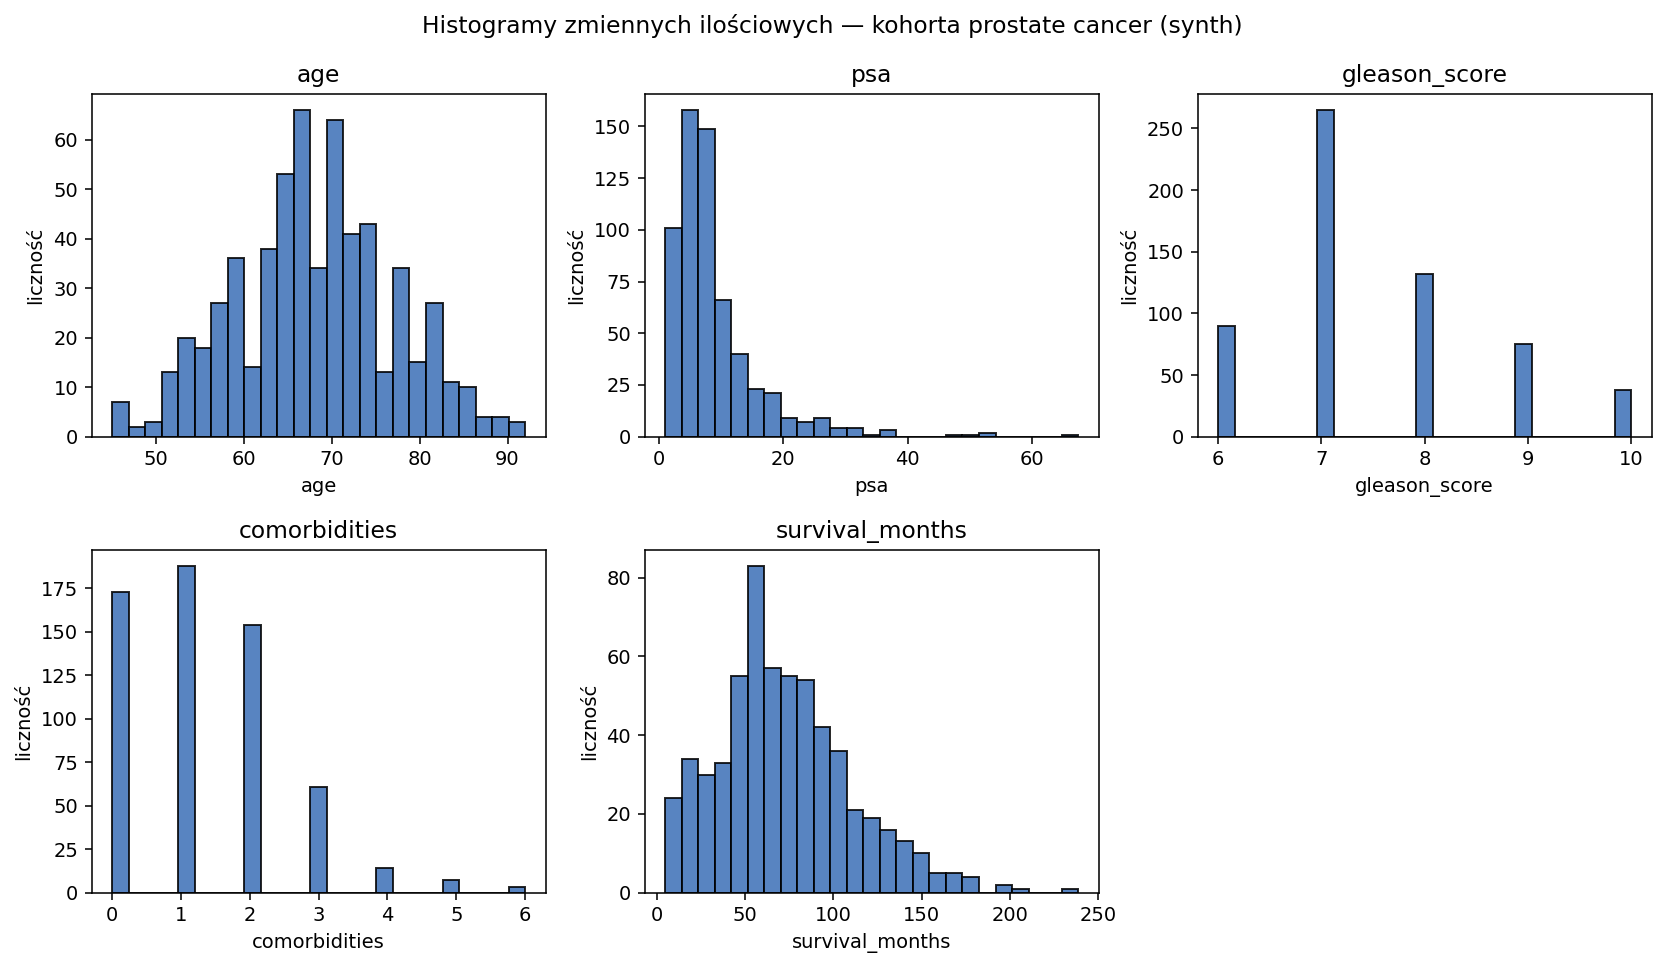
\includegraphics[width=0.85\linewidth]{hist_numeric.png}
\caption{Histogramy zmiennych ilościowych.}
\label{fig:hist}
\end{figure}
\begin{figure}[H]
\centering
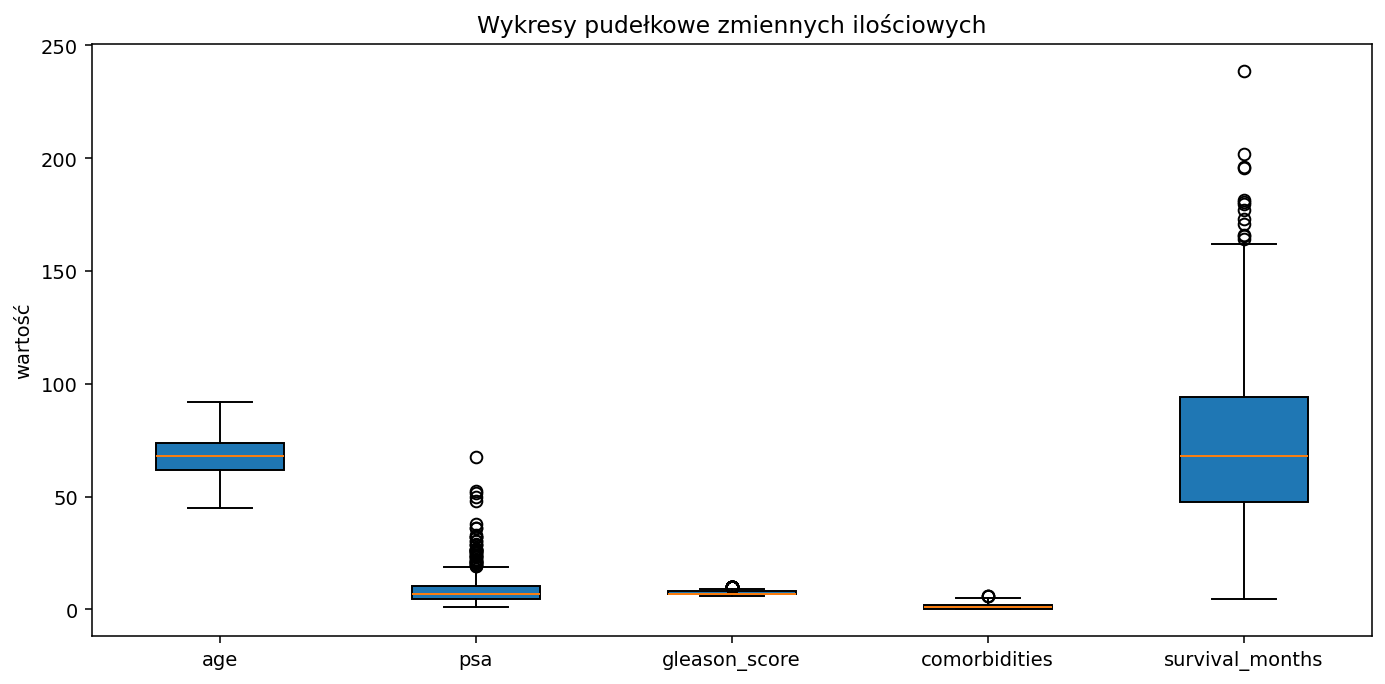
\includegraphics[width=0.85\linewidth]{boxplot_numeric.png}
\caption{Wykresy pudełkowe zmiennych ilościowych.}
\label{fig:box}
\end{figure}
\begin{figure}[H]
\centering
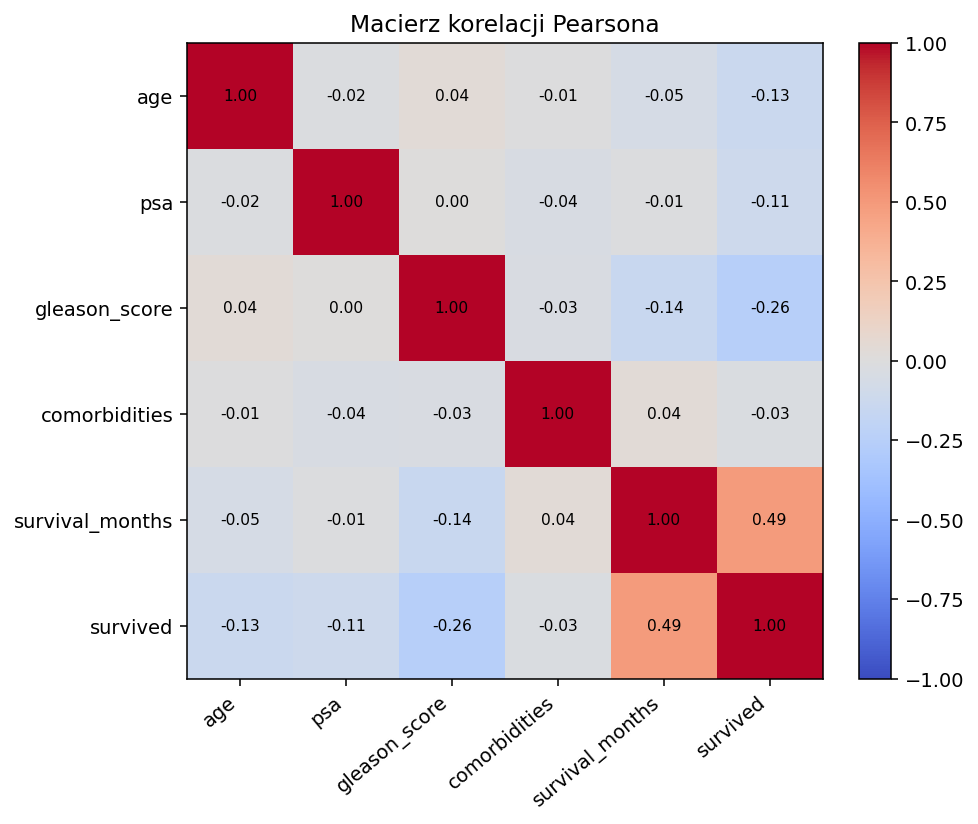
\includegraphics[width=0.85\linewidth]{corr_matrix.png}
\caption{Macierz korelacji Pearsona.}
\label{fig:corr}
\end{figure}
\begin{figure}[H]
\centering
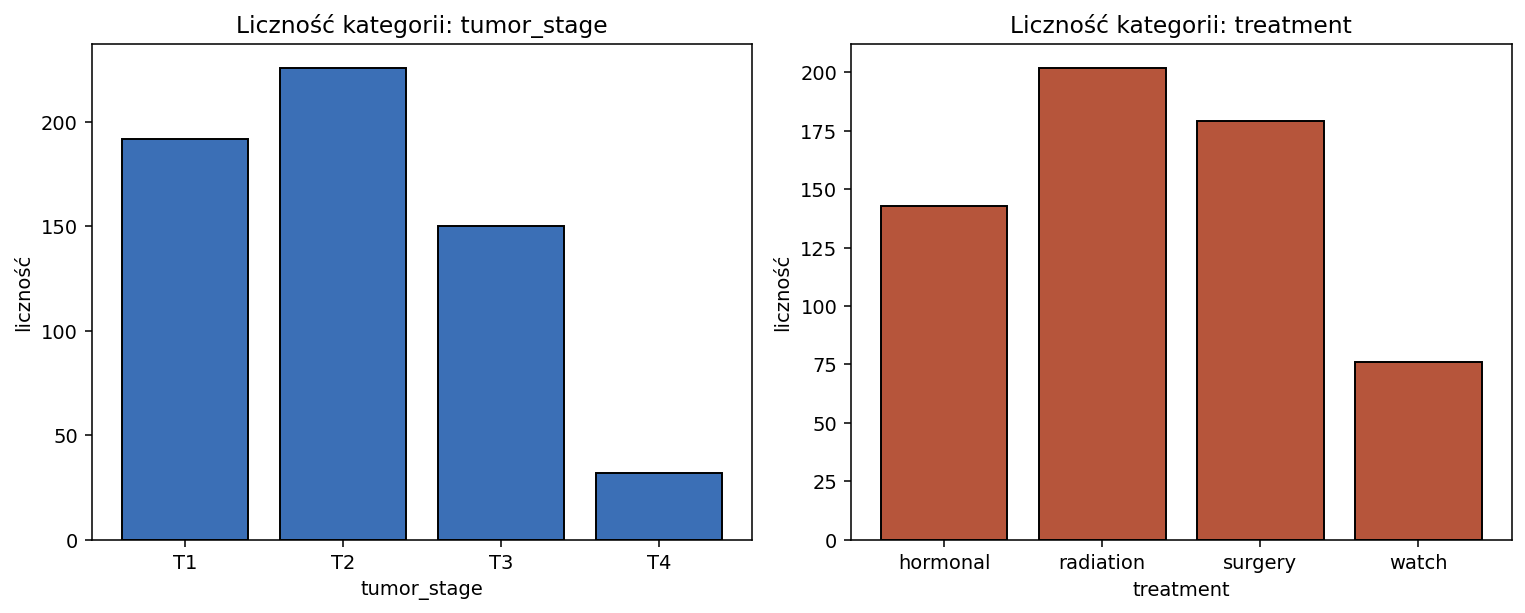
\includegraphics[width=0.85\linewidth]{categories.png}
\caption{Liczności kategorii \texttt{tumor\_stage} i \texttt{treatment}.}
\label{fig:cat}
\end{figure}


\section{Interpretacja wyników}
Histogramy pokazują typowe rozkłady: wiek skupiony wokół 68 lat, PSA prawoskośny (rozkład logarytmiczno-normalny), Gleason score skoncentrowany w okolicy 7. Macierz korelacji ujawnia umiarkowaną dodatnią zależność wieku i Gleason score z ryzykiem zgonu (ujemna korelacja ze zmienną \texttt{survived}). Liczności kategorii pokazują dominację stadium T1--T2 oraz terapii operacyjnej i radioterapii. Linia bazowa logistic regression osiąga AUC = 0.754, co potwierdza spójność danych i sensowność wybranych cech.

\section{Wnioski}
Etap importu, czyszczenia i analizy statystycznej został zrealizowany. Wprowadzono kontrolowane braki, które uzupełniono medianą bez utraty rekordów. Standaryzacja Z-score umożliwia porównywalność cech o różnych skalach. Analiza wskazuje, że PSA, Gleason score i stadium guza są informatywnymi predyktorami przeżycia, co stanowi punkt wyjścia dla bardziej zaawansowanych modeli (kolejne laboratoria).

\end{document}
